\begin{figure}[H]
	\centering
	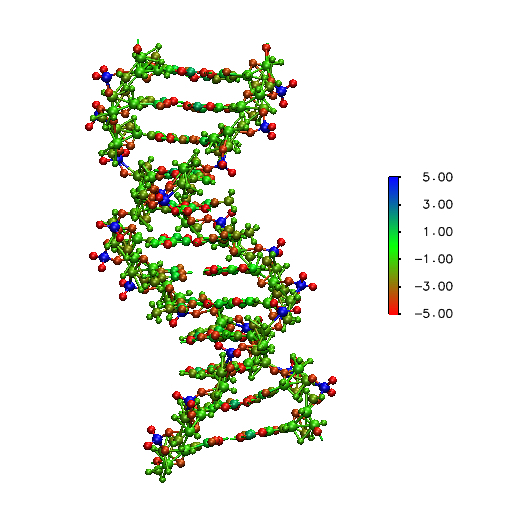
\includegraphics[scale = .5]{1bna_charge}
	\caption{Structure of a DNA (\textit{1bna}) constructed from its {\it .pqr} file showing atomic charges in color for each atoms.} 
\end{figure}
In order to calculate electrostatic potential and solvation free energy of real proteins,  we have to use the 3D structural data for proteins and nucleic acids available in the Protein Data Bank (PDB). PDB contains freely accessible data on the internet submitted by biologists and biochemists from around the world. These data are usually acquired by  X-ray crystallography, NMR spectroscopy, or, cryo-electron microscopy. Each molecule is represented by a unique name with four symbols, while each symbol could be either a letter or a number. Among several types of data file available from the PDB we focused on \textit{.pdb} type files available from the website of RCSB \cite{RCSB}, one of the member organizations of the PDB. Our goal here is to identify all atomic details of proteins, including the coordinates (x,y,z) of all atom centers, their van-der Walls radii, and partial charges assigned to each atom. 

\begin{table}[!t]
\begin{tabular}{|l|l|l|l|l|}
\hline
Record Type             & Columns & Data                            & Justification & Data Type  \\ \hline
\multirow{15}{*}{ATOM}  & 1-4   & “ATOM”                          &               & character  \\ \cline{2-5} 
                        & 7-11  & Atom serial number              & right         & integer    \\ \cline{2-5} 
                        & 13-16   & Atom name                       & left         & character  \\ \cline{2-5} 
                        & 17      & Alternate location indicator    &               & character  \\ \cline{2-5} 
                        & 18-20  & Residue name                    & right         & character  \\ \cline{2-5} 
                        & 22      & Chain identifier                &               & character  \\ \cline{2-5} 
                        & 23-26   & Residue sequence number         & right         & integer    \\ \cline{2-5} 
                        & 27      & Code for insertions of residues &               & character  \\ \cline{2-5} 
                        & 31-38   & X orthogonal Å coordinate       & right         & real (8.3) \\ \cline{2-5} 
                        & 39-46   & Y orthogonal Å coordinate       & right         & real (8.3) \\ \cline{2-5} 
                        & 47-54   & Z orthogonal Å coordinate       & right         & real (8.3) \\ \cline{2-5} 
                        & 55-60   & Occupancy                       & right         & real (6.2) \\ \cline{2-5} 
                        & 61-66   & Temperature factor              & right         & real (6.2) \\ \cline{2-5} 
                        & 73-76   & Segment identifier              & left          & character  \\ \cline{2-5} 
                        & 77-78   & Element symbol                  & right         & character  \\ \hline
%79-80                   & Charge  &                                 & character     &            \\ \hline
%\multirow{2}{*}{HETATM} & 1-6   & “HETATM”                        &               & character  \\ \cline{2-5} 
%                        & Jul-80  & same as ATOM records            &               &            \\ \hline
%\multirow{6}{*}{TER}    & 3-Jan   & “TER”                           &               & character  \\ \cline{2-5} 
%                        & 7-11  & Serial number                   & right         & integer    \\ \cline{2-5} 
%                        & 18-20  & Residue name                    & right         & character  \\ \cline{2-5} 
%                        & 22      & Chain identifier                &               & character  \\ \cline{2-5} 
%                        & 23-26   & Residue sequence number         & right         & integer    \\ \cline{2-5} 
%                        & 27      & Code for insertions of residues &               & character  \\ \hline
\end{tabular}
\caption{Protein Data file (\textit{.pdb} type) format}
\label{tab:PDB_format}
\end{table}
%TODO have to describe the format of pdb file then apbs type the pqr type. 

 In a \textit{.pdb} file for a particular protein, ATOM record type (the rows starting with the word "ATOM") contains the information about each atom as shown in Table \ref{tab:PDB_format}. This raw information is not readily usable for our proposed solver. A Python script has been developed to follow the following steps,


%\begin{enumerate}
\begin{itemize}
 	\item Reading \textit{.pdb} file RCSB website: The Python module \textit{"requests"} has been used to read and parse protein data from the web from the web address 'https://files.rcsb.org/view/' to write a local \textit{.pdb} file. 
	\item Converting  local \textit{.pdb} file to \textit{.pqr} file: The PDB2PQR software \cite{PDB2PQR} has been used to calculate the {\it .pqr} file. These \textit{.pqr} files contain ATOM record types similar to \textit{.pdb} files where the occupancy columns (55-60) and Temperature factor columns (61-66) have been replaced by the charge and radius.     
	%\item Parsing ATOM record types to collect $X,Y$ and $Z$ cor
 \end{itemize}
% \end{enumerate}

Finally in \textit{.pqr} files we have the $X,Y$ and $Z$ co-ordinates, the charge of the atomic center and the radius for each individual atom.  